\section{实验:研究弹簧秤的刻度}\label{sec:2-5}

\shiyan{目的} 研究弹簧的伸长跟拉力的关系,了解弹簧秤刻度的原理。

\shiyan{器材} 铁架台,木条,白纸条,下端带指针和挂钩的弹簧,四个质量相等的钩码,刻度尺,夹子,弹簧秤,待称的物体。

\shiyan{步骤}

(1) 把白纸条拉直,两端贴在木条上。用夹子把木条竖直固定在铁架台上。把弹簧挂在支架上(参看图 \ref{fig:2-8})。
待弹簧静止后在白纸条上用短横线记下指针的位置。

(2) 把钩码轻轻地挂在弹簧上。先挂一个,再挂 2 个,3 个,4 个。每挂一个钩码都用短横线在白纸条上记下指针的位置。
最后把钩码全部取下来,看看指针是否回到原来的位置。

(3) 取下白纸条,在纸条上标度。如果你所用的钩码每个的质量是 50 克,那么根据 $G = mg$,
一个钓码重 $0.49$ 牛顿,两个钩码重 $0.98$ 牛顿 …… 把各次悬挂的钩码重写在纸条上对应的横线旁,
再在最上面一条横线旁写上“0” 。

(4) 用刻度尺依次量出白纸条上各条横线到“0”线的距离 $\Delta l_1$、$\Delta l_2$、$\Delta l_3$、$\Delta l_4$,
并根据各条横线对应的钩码重,研究弹簧的伸长是否跟拉力成正比。

(5) 把白纸条贴回原来的位置,也就是使弹簧不挂物体时指针对着纸条的“0”线,我们就可以用这根弹簧来称物重了。
把待称的物体挂在弹簧上,从指针的位置读出它重多少。

(6) 用弹簧秤测出待称的物重,把它跟 (5) 中的结果相比较。

\shiyan{注意事项}

(1) 实验中不可用力猛拉弹簧,以免损坏。

(2) 在白纸条上画横线时,视线要跟指针在同一水平面上。

\shiyan{思考题} 弹簧秤的刻度为什么是均匀的?


\nonumsection{小制作:自制橡皮筋测力计}

\begin{wrapfigure}[14]{r}{4cm}
    \centering
    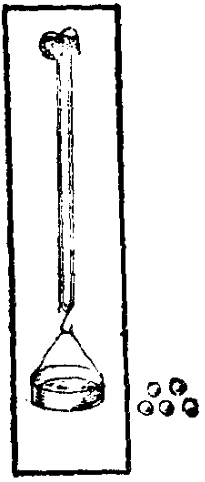
\includegraphics[width=0.2\textwidth]{../pic/czwl1-ch2-10}
    \caption{}\label{fig:2-10}
\end{wrapfigure}

用像皮筋(一条或几条),几个大小相近质量已知的玻璃弹球或泥球,一条硬纸板,一个小盒盖,自制一个简单的测力计(参看图 \ref{fig:2-10})。
用它称出钢笔、橡皮、铅笔盒各重多少。再用弹簧秤称一称,看看你的测力计做得怎样?你的测力计的刻度是均匀的吗?如果不均匀,这说明什么?


\nonumsection{阅读材料:物重和质量}

我们已经学过了物重和质量,这是两不同的物理量。
它们的物理意义不同,质量是物体所含物质的多少,物重是由于地球的吸引使物体受到的力。
它们的单位不同,质量的单位是千克,物重的单位是牛顿。
测量质量和物重的仪器也不同,质量用天平测量,物重用弹簧秤测量。

但是在日常生活中,人们对物重和质量常常不方区别,而把质量当作物重。例如,我们买粮食是为了从粮食中吸收养物质,
所以关心的是物质的多少,但是习惯上却把买质量为多少千克的面粉说成重多少千克;我们查身体是为了了解肌肉、骨胳
以及各个器官的发育是否正常,所以关心的也是质量,但是习惯上总是把称得的身体质量是多少千克说成体重是多少千克。

因为质量为 1 千克的物体,在地球上受到的重力为 1 千克力,所以在用千克力作重力单位的时候,质量为几千克的物体,
它就重几千克力,即质量的数值与重力的数值是相等的。但是必须注意,只有在地球上物体质量的千克数跟它受到的重力的
千克力数才是相等的。如果到了月球上, 物体由于被月球吸引而受到的力也叫重力,而月球对物体的吸引力只有地球的六分
之一,所以质量为 1 千克的物体,在月球上受到的重力就不是 1 千克力,而是 $\dfrac{1}{6}$ 千克力了。
一名能举起 100 千克杠的运动员,在世界比赛中是得不到名次的。是假如他到了月球上,他就能举起质量是 600 千克的杠铃,
而 1981 年世界举重锦标赛中,力气最大的冠军才只举起 $201.5$ 千克。

\begin{figure}[H]
    \centering
    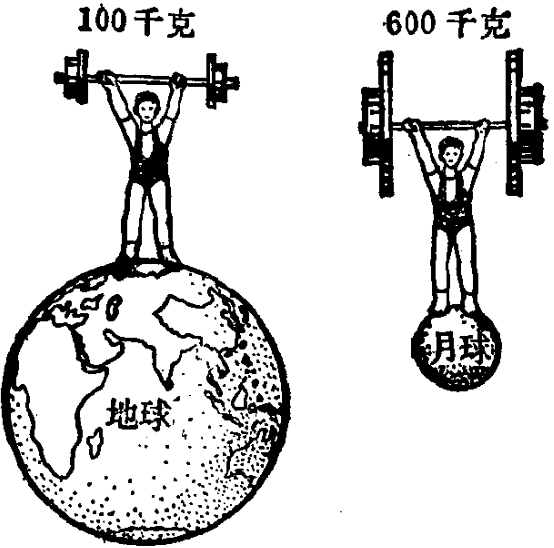
\includegraphics[width=0.4\textwidth]{../pic/czwl1-ch2-11}
    \caption{}\label{fig:2-11}
\end{figure}

